\documentclass {report}
\usepackage{graphicx} 
\usepackage{indentfirst}
\graphicspath{{images/}}
\usepackage[a4paper,left=3cm,right=2cm]{geometry}
\usepackage{url}

\begin{document}
%\begin{titlepage}
%\title{%
%Application of Cloud Computing for Sensor Network}
%\author{%
%Dr. Mahmuda Naznin Madam\\
%Bangladesh University of Engineering and Technology}
%\maketitle

%\end{titlepage}


\begin{center}\textbf{{ \Large A Survey on Application of Cloud Computing for Sensor Network\\ }
Submitted To-Dr.Mahmuda Naznin \\ Submitted By - Anjana Tiha \\Student No - 0505071
\\Department of Computer Science and Engineering \\ 
Bangladesh University of Engineering and Technology }\\  \end{center}


\begin{abstract}
A sensor network consists of sensors that spread out several hundred instances,which sample the physical data of the environment.
The data is stored temporarily in local nodes and transmitted to the sink node.This new network can deliver several applications that create valued services for consumers.
Cloud computing renders publicly available, elastic and dynamic computing architecture.Users can freely select various levels of cloud platforms from Software as a Service (SaaS), Platform as a Service (PaaS) to 
Infrastructure as a Service (IaaS).The scalable computing power for data analysis, active application development tools and a virtually infinite capacity for storage make cloud computing technically alluring for sensor data integration.
The parsing and processing of data is very easy.Cloud also acts as a library with elastic capacity in which users only need to put effort in developing the application features while underlying structure is hidden. 
Geographically distributed data centers ensure data safety by programming regular replication of data to a different data center.\\

\end{abstract}


\tableofcontents


\chapter {Introduction}
Cloud computing is a computing concepts that involve a large number of computers connected through a communication network such as the Internet [11].Physical resources like computer, storage, networking capacity are shared using high level of abstraction where physical devices simulate virtual devices.The resources can be shared among multi-tenant.
The Cloud Computing technology is applied in many spheres, including, scientific computation, e-commerce, online games,virtualization of office documents.The core 
features of Cloud Computing  include cost-effectiveness, elastic resource allocation, 
virtualization and pay-per-use pricing models.
Wireless Sensor network consists of  sensory devices that collect raw enviornmental data from nearby location and connect to each other and center node by wireless signal. But WSNs(Wireless sensor networks) have limitations: 
\begin{itemize}
\item  Limited computational resources 
\item Low battery power
\item Heterogeneous  devices
\item Short life
\item Costly installation of devices
\end{itemize}
The complementary characteristics of Cloud Computing and WSNs is an indication to the advantage of this two technology.\\


\section{Cloud Computing}

Cloud computing is becoming increasingly popular in today's world.Both end users and 
developers are growing more interested in cloud computing technology. 
Cloud Computing network consists of virtually simulated machines that provides on demand services with rapid scalability and considerable storage facility.It provides 
immense amount of resources which is impossible in previous solutions for computing 
and data storage.\\
 It is a way of incorporating a set of technologies to 
implement a new system that creates a ground for users to have access to shared 
and configurable computing resources through internet on-demand.The resources that
are commonly shared are storage networks, servers, application that can be provisioned 
with ease and minimum interaction with the service provider.\\
This new paradigm has allowed 
end users to access variety of services without going through the trouble of hardware and 
software management. The service provider is solely responsible for installation, back up,
storage maintenance, application and software management with security for data provided
on the network. This enables organizations to invest more resources on their core business
than maintaining and managing the IT related problem.\\
From current trend of cloud computing the following aspects have been Recognized:\\

{\bfseries Shared Infrastructure:}

The technological resources of cloud service providers are combined to serve multiple
consumers with different physical and virtual resources dynamically assigned and reassigned
on demand [12].The consumers actually have no knowledge of the exact location of the provided 
services but one can specify and limit their data to some specific locations upon request to the 
service provider.Otherwise the shared data is available from any location where cloud network
can be accessed.\\

{\bfseries Broad Network Access:}

This feature makes it possible to access the services from any location through internet
with broad range of devices including light technology like mobile, tablet, PC and laptop.\\

{\bfseries Rapid Elasticity:}

The service capability can be provisioned based on demand been placed on [12].When additional
resources required on end user level, cloud infrastructure can quickly grow and expand the
allocated resources to meet additional demand.Further resource preoccupation is released 
when the demand has been dropped.This automated resource management makes the
distribution of capability more efficient by ensuring that no user has more resource than
needed.\\

{\bfseries Highly Abstracted:}

The end consumers don't need to manage the hardware, storage or the software [12].The 
whole system is highly abstracted and the underlying structure is securely obscured from the user.
The cloud owners avoid revealing their solution as it is their part of strategic
information.Although some academic and non academic researchers are trying to develop 
open source clouding solutions.\\

\subsection{Cloud Services Architecture}

Services provided by the cloud computing system includes 3 basic types:

{\bfseries Software as a Service (SaaS) providers:\\}
SaaS is a multi tenant environment to provide single or a few services to the users.
Service is offered on demand and as per use method.They appeal to clients that need 
on demand services rendered by an external provider who handles underlying software
and hardware.Some service provider own the data center while others render services
from other cloud providers [12].\emph{ Example - SalesForce.com,Google Mail,Google Docs}\\

{\bfseries Infrastructure as a Service (IaaS) providers:}
IaaS provides the backbone of cloud computing.They render storage, processing power,
network capacity and other hardware resources as service.Customers can directly access
the infrastructure as pay per method.High level abstraction is used to obscure the real 
hardware from consumers.Real Machines simulate virtual machines.The customer can use
hardware resources on virtual level [12].The process of abstraction can help the user grow and
expand services according to the need.\emph{ Example-Gogrid mozo/rackspace, flexiscale, Amazon's EC2.\\}

{\bfseries Platforms as a Service (PaaS) providers:\\}
PaaS provides professionals with platform to develop simulate and run application on server
without needing to handle underlying hardware system.Paas has the same capability as
the on-premises application server.The cloud server hold both completed and in-progress
applications.Users can build their software for own use or for commercial purposes.They
only have to pay for the resources they used and due to service scalability service capacity 
can be enhanced immediately on demand [12].As the infrastructure is shared the platform cost
very much less compared with otherwise solutions.\emph{Example- Google App Engine is such an example.\\}

\begin{figure}
%\centering
\begin{center}
\includegraphics [scale=0.3]{as}
\caption{Services Provided By The Cloud Computing System}
\end{center}
\end{figure}


\subsection{Open source Solution For Cloud}

Cloud computing has some open source solutions available.

\subsubsection{Xen Cloud Platform (XCP)}
Xen Cloud Platform is used by other cloud solution.Xen Hypervisor does not offer the
whole infrastructure for the cloud computing solution like Nimbus, Amazon EC2 and 
Eucalyptus.It mainly provides the service of automation of the process and 
maintenance for platform.Hypervisor Provides virtualization giving abstraction 
between the hardware and the operating system.Each physical machine can run
several virtual machine hiding underlying system and application.\\


\subsubsection{Nimbus}
Nimbus is an open source solution that turn clusters into an Infrastructure 
as a Service (IaaS) for scientific applications. 
This solution gives the customers the additional benefit of allocating and configuring
resources.
This solution gives to users the benefit of allocating and configuring remote 
resources by deploying VMs – known as Virtual Workspace Service (VWS).A VWS is 
a VM manager that different front ends can invoke. \\

\emph{Workspace Service}: Provides security with authentication and authorization.\\
\emph{Workspace Pilot}: Delivers the service of vitualization of the system with some additional handling of administrative work.\\
\emph{Workspace Control}: Responsible for controlling virtual machines, assigning IP and mac addresses and reconstructing images.\\
\emph{Workspace Resource Management}: Used to control different VM machines.\\


\section{Sensor Networks}
In a sensor network sensors are spatially distributed across the network.They are deployed to take non heterogeneous information from places of potential threat, hazard prone and remote and in mining area.In it's youth, sensors were used
for battleground surveillance.Sensors are small devices with embedded program and built-in radio/wireless transceiver,power source and CPU.The sensors keep track of various environmental data
and does aggregation and prepossessing before the data is sent to central node called sink. The nodes can be connected to each other or directly to the sink or both ways.The sink does complex calculation and analyze the data to 
provide the required information of the sensor network and environment.\\
\indent The development of technologies in WSN arena requires development in three areas- sensing, communication,  computing.The researchers have focused on in-network support for wireless sensor network which has resulted in development 
of tiny OS that support WSN.\emph{eg. tinyOs, contiki}.\\
\indent Researchers are also working on developing a level of abstraction for WSN which include specialized component models such as NesC, OpenCom along with macro-programming approaches
such as TinyDB.There have been prolific improvement in network support for WSN from network layer to application layer.
The sensors are small in size cost less energy but shortcomings of sensors like low computing capacity,limited memory and low power battery makes complex data services difficult to provide.\\


\subsection{Routing Technology}
The routing technology is divided into two categories:
\begin{itemize}
\item Network Structure Based 
\item Protocol Operation Based
\end{itemize}

\begin{figure}
%\centering

\begin{center}
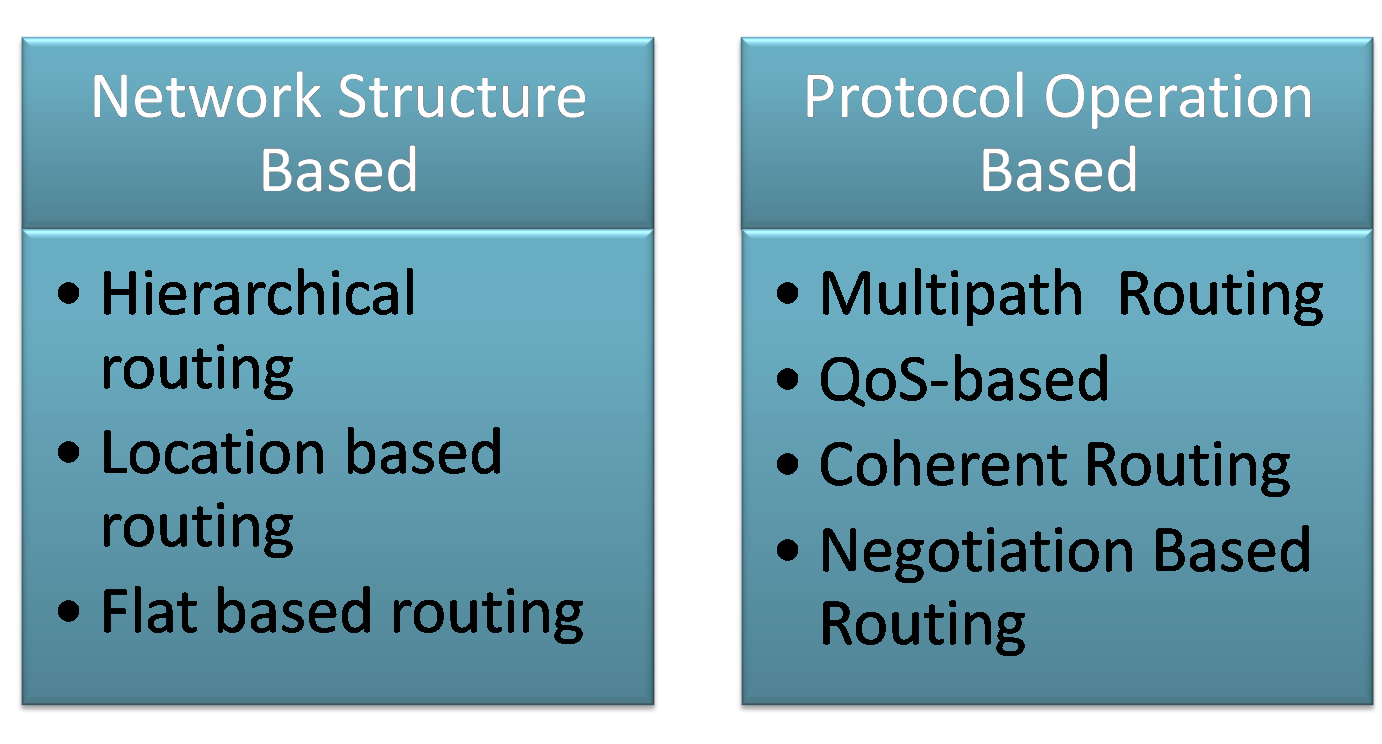
\includegraphics [scale=0.3]{images/rou}
\caption{Routing Technology}
\end{center}
\end{figure}


\subsubsection{Network Structure Based}
There are different routing algorithms that implement \emph{Network Structure Based Routing}.\\

\emph{{\bfseries Flat Based Routing:\\}}
In flat based routing all the nodes are assigned similar roles of performing the task of sensing by collaborating [12].Since flat based routing has a very large number of sensors, it is not efficient to assign global identifiers.As all the nodes have to perform all the tasks, 
the work load of sensing, computation and communication is significantly high which is not energy or cost efficient.\\

\emph{{\bfseries Hierarchal Routing:\\}}
Hierarchical routing is a two layer routing, one layer used to select cluster head and other layer for routing.All the nodes in the network are grouped into clusters [12].Each cluster has a cluster head which is also a sensor node.Low energy
Cluster member nodes does the sensing in proximate target and cluster head does the computation and communication.This system is more energy and cost efficient, largely scalable.Data aggregation and data fusion is applied on data in member nodes.
This produces energy and cost efficient solution and reduces the transmission load on network.\emph{Example-LEECH, TEEN\\}

\begin{figure}%FIGURE
%\centering
\begin{center}
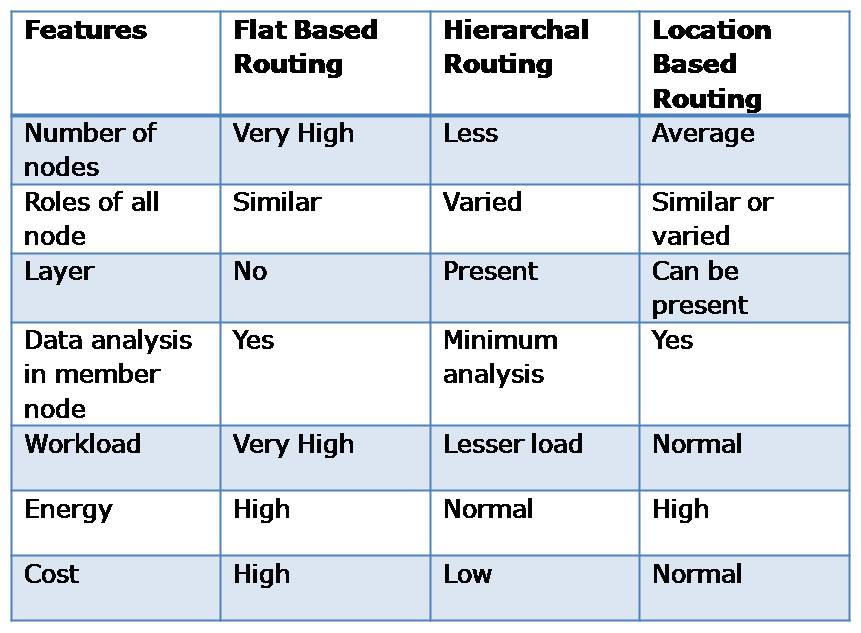
\includegraphics [scale=0.5]{table1}
\caption{Network Structure Based Routing}
\end{center}
\end{figure}

{\bfseries Location Based Routing:}
In this model the location of the nodes are exploited [12].They are addressed by their location.The distance can be calculated by analyzing signal strength and relative distance can by calculated by exchanging information between nodes.\\

\subsubsection{Protocol Operation Based}
\emph{{\bfseries Multipath  Routing:\\}}
The routing protocol uses multi-path instead of single path.\\
\emph{{\bfseries QoS Based  Routing  Protocol:\\}}
The network  has to balance  between energy consumption and data quality.Network has to satisfy certain QoS terms, e.g. energy,  delay, bandwidth etc  for  delivering  data [12].\\
\emph{{\bfseries Coherent Routing:\\}}
The data is forwarded after minimum processing that includes time  stamping, duplicate  suppression,  etc.\\
\emph{{\bfseries Negotiation Based Routing:\\}}
The protocol eliminate redundant data transmissions through negotiation.Communication decisions are taken based on the available resources.\\

\begin{figure}
%\centering
\begin{center}
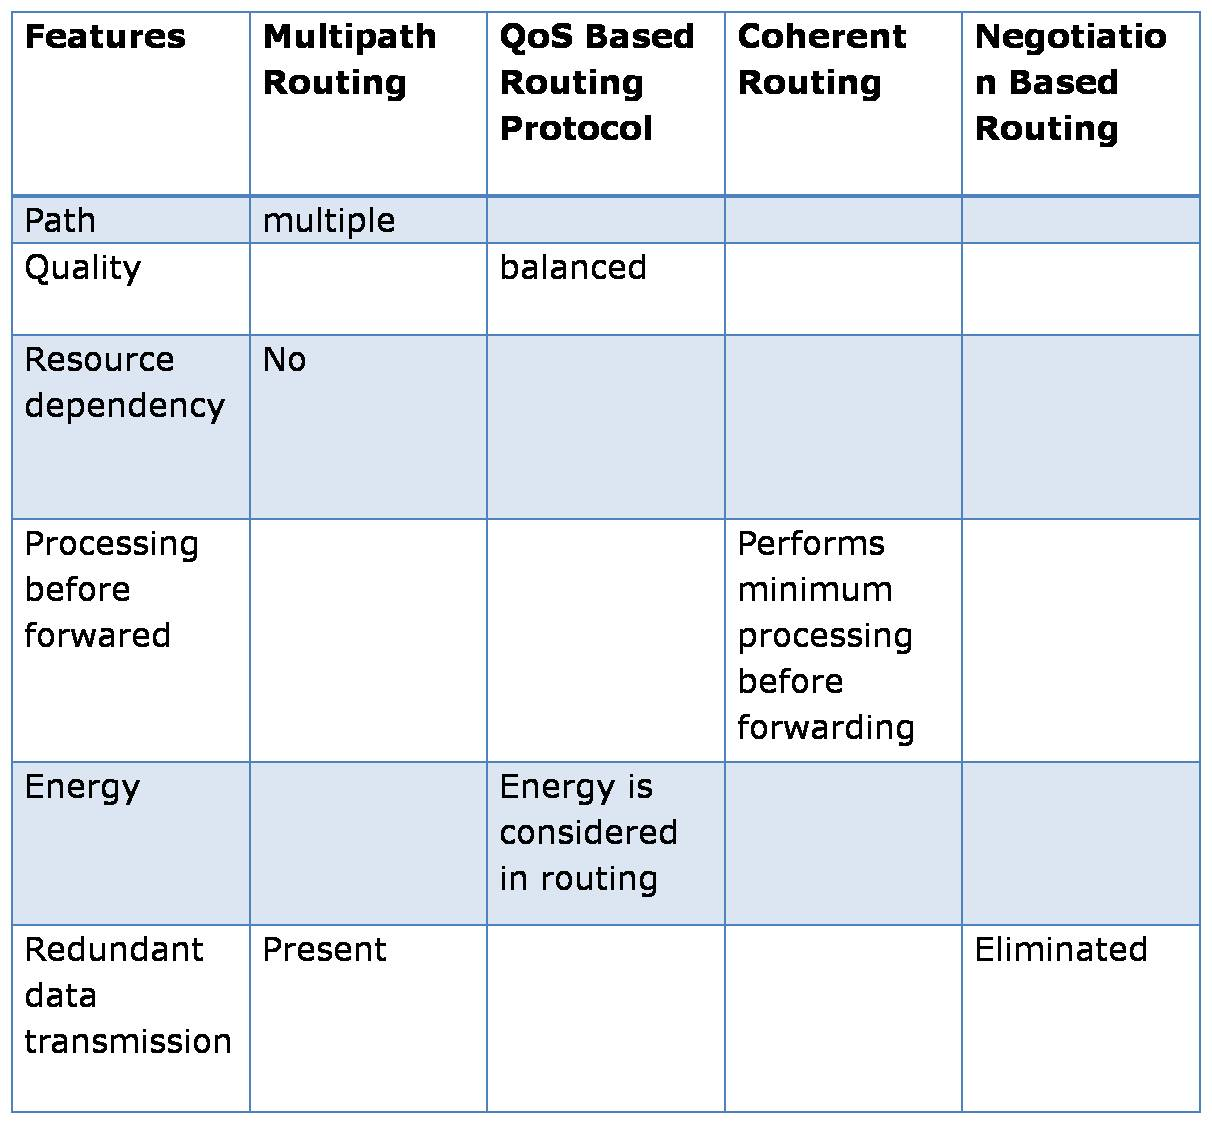
\includegraphics [scale=0.3]{table2}
\caption{Protocol Operation Based Routing}
\end{center}
\end{figure}


\chapter{Related Works}

\section{Haddop Cloud solution for Wireless Sensor Network}


In this architecture Googles Cloud Solution Hadoop is adopted as cloud solution of the architecture.We also propose a new way of sensor organization in a zone [4].The homogeneous sensors form a WSN, while heterogeneous 
sensors form logical independent but physically overlapped WSNs.Sensors could be managed by the cloud through sink point.

\subsection {Architecture}

All nodes are divided into cluster or zone.A number of sink points(cloud node) are distributed across the WSN area to form a cloud. We refer this type node as “cloud node”, after processing data from sensors, 
cloud can assign nodes to perform properly.The cloud can control activities of a sensor timely based on data collected from the whole WSN as the whole network is divided into smaller zones.

{\bfseries Sensor Network:}\\
 All The sensor nodes are divided into many zones, with each zone theres a virtual sink point.Cloud acts as the sink and accumulates sensing data of different zones.Multimedia sensor network (WMSN) consisting of
 powerful sensors, for example, image sensor, audio sensor, video sensor, etc., are employed to capture rich information of the area
WMSN requires more resources for handling large data.\\
\indent Various techniques are used to alleviate resource storage limitations.The common strategies are-Data compression, efficient image data coding,
cross-layer communication protocols, smart activity scheduling, and energy-efficient routing techniques.Optimization techniques are used in all the layers to reduce energy consumption
Data in cloud are stored and processed in distributed manner,which would be preferred for large volume data process as it facilitates parallel processing.\\

\begin{figure}
%\centering
\begin{center}
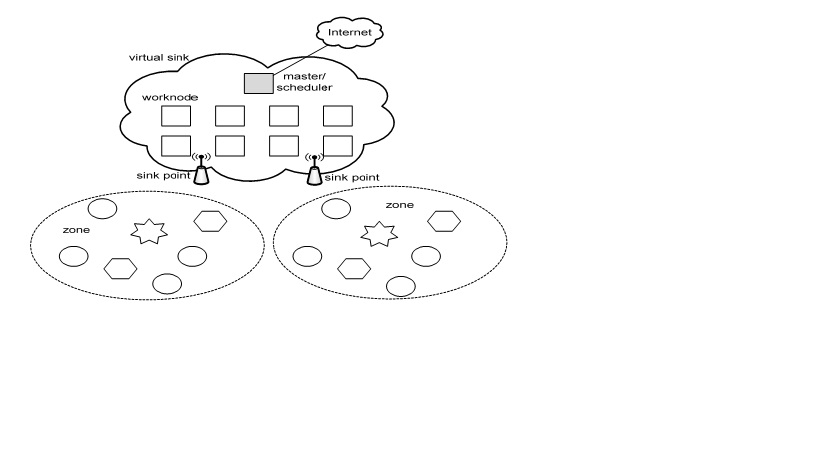
\includegraphics [scale=0.7]{Hadoop}
\caption{Cloud computing based WSN architecture[4]}
\end{center}
\end{figure}

{\bfseries Organizing Cloud:}\\
Hadoop is intended for big data storage and processing tasks.Data movement reduction is one of its special.This architecture proposes  master-slave structure for storage and data processing.Master is
responsible for storing file meta data and scheduling tasks and slaves are responsible for storing file content or job execution.The two masters could be placed either in the same or in different physical nodes.
The master node is linked to the internet.A cloud node is slave of the Hadoop cloud, and also the sink point of a zone.It receives data sent by sensors in the zone and then acts as a client to store the data into Hadoop. \\

\section{Extending Sensor Networks into the Cloud using Amazon Web Services}
%Kevin Lee
Amazon Web Services (AWS) is cloud computing architecture provided by amazon which offers Elastic Computing Cloud (EC2),Simple Storage Service (S3) and SimpleDB and MapReduce[10].Amazon Web Services
can be accessed through using web browser or client application tools [10].\\
\emph{{\bfseries EC2}} : provides support for the dynamic instantiation and configuration of virtual machine instances.\\
\emph{{\bfseries S3}} : provides support for creating and managing an extensible storage space of heterogeneous data.\\
\emph{{\bfseries SimpleDB}} : provides support for setting up simple relational databases that allow developers to store and query data without database management.\\
\emph{{\bfseries Elastic MapReduce}} : provides support for performing data-intensive tasks with minimal setup and management overhead.\\
\indent Together, the AWS suite of services provides rich support for the creation and management of elastic computation facility.The provision of sensing resources in the Cloud extends the current 
domain of Cloud Computing to include the physical world. We refer to this vision as the Tangible Cloud.\\

\begin{figure}
%\centering
\begin{center}
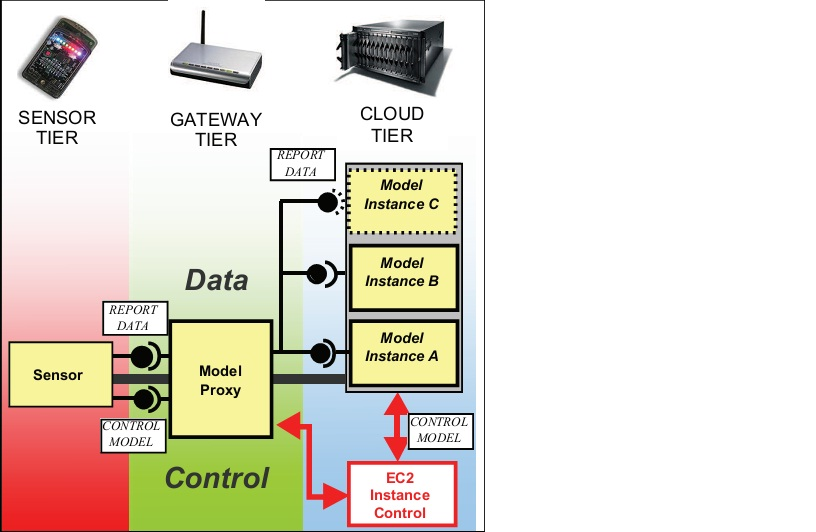
\includegraphics [scale=0.5]{amazon}
\caption{System Overview[10]}
\end{center}
\end{figure}

\subsection{The Sensor Tier Architecture}
The environmental data is gathered on sensor nodes running the LooCI [10]. Sensing functionality is achieved using generic LooCI components. Both the data and control plane are accessible in-network
 over the event bus.The model proxy offers LooCI interfaces to control the extensible model and report data. This eliminates the need to provide in-network adapters and thus lowers overhead.\\

\subsection{The Gateway Tier Architecture }
The Model Proxy acts as a bridge, allowing LooCI sensing components to parameterize the extensible mode [10]. Additionally, the model proxy relays environmental sensor data from the sensor network to the most optimal model instance.\\ 

\subsection{The Cloud Tier Architecture }
An extensible model is realized as an Auto Scaled set of EC2 instances. Each model is implemented in LooCI and therefore may connect directly to the model proxy over the event bus. Model functionality
is encoded in a pre-configured EC2[10] AMI image and when the current pool of instances approaches a CPU utilization trigger [10], a new instance can be dynamically instantiated.Once it is instantiated, 
a reference is passed to the model proxy, which includes the instance in the Model pool, providing new capacity.Additional Capacity may also be added manually.\\
 
\begin{figure}
%\centering
\begin{center}
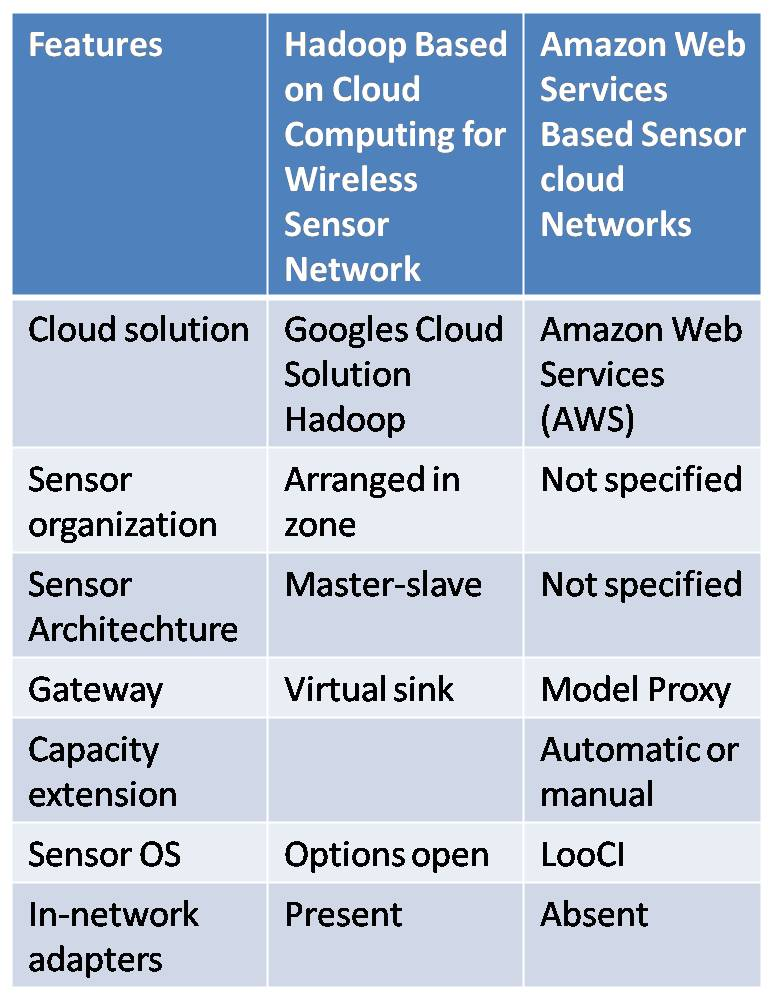
\includegraphics [scale=0.6]{architecture}
\caption{Comparision Table}
\end{center}
\end{figure}
%\newpage


\chapter{Proposed solution for Integration}

\section{Architecture}

\subsection{Sensor Organization}

Sensors of homogenous nature are clustered into one group and heterogeneous sensors may form different cluster. Each cluster will have a gateway sink point which will help two way communications between sensor and cloud in direct manner. Sensors with heavy data load uses different gateway than normal sensors.The sensor capabilities will be parameterized by installed application and facilitate the user access and control of sensing activities.Sensors in a cluster may be interconnected to form global picture of the 
enviornment.Hierarchical or QoS routing may be adopted in sensor connectivity.\\

\subsection{Virtualization}
Sensors used in the network may be heterogeneous in kind.They will be scattered in different locations.The OS used in sensors can vary so does the physical capability and specification.It is much convenient to handle the sensor from remote places using cloud app developed for sensor network than controlling from actual physical location.This solution is more convenient than relentless sensor data transmission.So redundant data transmission can be avoided by direct administrative handling of devices. Sensor device handling will require a level of virtualization for sensor device safety.One can create virtual device from physical sensor.\\

\subsection{Standardization }

Sensor will be of different kind and the collected data will be of heterogeneous nature.The operating system the sensors will be running on may not be the same. So handling of sensors will require virtualization along with standardizing of the sensor handling. Authorized administrative users can control and access all sensors in Standard method without concerning device specifications loud will translate the uniform access and control functions into device specific function.
Virtualization will abstract the sensor resources to and manage these resources according to terms and conditions.To run different application in sensor run time environment has to be installed.\\


\subsection{Actors on the System}

{\bfseries Cloud owner:}
Cloud owner has overall infrastructural control and access.Cloud owner is responsible for physical maintenance of the system and virtualization and management of IT resources.

{\bfseries System Owner:}
System owner rents cloud and sensor capabilities and has overall ownership of all data, sensor control and app maintenance.

{\bfseries Administrative Use:r}
Administrative user is the actor that has access to raw data of sensors The database control and access is strictly limited to only this type of user. Sensor app developer and service maintenance engineer fall into this group.

{\bfseries End User:}
 End user is a system actor with one or more application and services to that capitalize on sensor data.User can control and access sensors via web browser.Sensor data collection and analysis is aimed primarily for end user service. Developed apps based on sensors provide service to the end user.


\section{Mobile As Sensing Device}
Mobile phone is maturing as computational platform with added functionality of sensors [3]. Mobile sensing is another new concept.
Mobiles are equipped with embedded sensors such as g- sensor, E-compass, Gyroscope, Light Sensor, Proximity Sensor, Accelerometer(aka G-sensor), video camera, GPS, Wifi 3G/4G radios, microphone.\\
{\bfseries {\small Accelerometer(G-sensor):}}
G-sensor senses acceleration (with high-pass filter) and gravity vector.\\
\emph{Available}: Found in all smart phones.\\
\emph{Application}: Gaming.\\
{\bfseries {\small E-compass:}}
Senses magnetic field for mid-range and high-end smart phone.\\
\emph{Application}: Compass and GPS.\\
{\bfseries {\small Gyroscope:}} Senses angular momentum.\\
\emph{Available}: High-end smart phone.\\
\emph{Application}: Gaming.\\
{\bfseries {\small Light Sensor:}} 
Used to adjust brightness of the screen.\\
\emph{Available}: All smart phones.\\
\emph{Application}: Controls display brightness based on based on ambient light present.\\
{\bfseries {\small Proximity Sensor:}} Senses nearby objects.\\
\emph{Available}: All smart phones.\\
\emph{Application}: Prevent unwanted touch-input when user's ear is near to the phone.\\

All the sensing applications can be used to detect different type of environmental and user data from the mobile phone.Data collected from mobile can be used to reach decision about the environment.
Mobile phone sensing can be used to bring automation in e-health, traffic sector etc.
Mobile can upload the data on cloud computing platform based on contract and terms.From cloud, other users can use the data to get desired services.\\

\subsection{How it Works}
Multiple sensing servers can be deployed to manage sensing requests from different locations.When a cloud user initiates a sensing request through an online
application form in a web server from devices,the request will then be forwarded to a sensing server which will then push the request to a subset
of mobile phones that is located in the respective area.The sensing request will be fulfilled by these mobile phones.The sensed data will be collected by a server then stored in the database and will be returned to the cloud user.
Cloud user can not only request the service but also is someone who fulfills sensing request.\\

Two model of Mobile Sensing:
\begin{itemize}
\item Participatory Sensing
\item Opportunistic Sensing
\end{itemize}

{\bfseries \emph{Participatory Sensing:}\\}
	User can actively engage in sensing activities and determine manually the sensing actions.Sensing service management is distributed among users.\\
{\bfseries \emph{Opportunistic Sensing:}\\}
	System is fully automated without user participation.The process is controlled by a single organization.\\

\subsection{Limitation of Mobile Sensing:}
\begin{itemize}
\item Mobile sensing is a power greedy service to offer.
\item User needs varying incentive in return of mobile sensing and data service.
\end{itemize}

\section{Application of Cloud Computing For Sensor Network}
Integration of WSNs with cloud makes it easy to store, share and analyze real time sensor data with very high processing capacity.This technology can introduce new terminology called sensing as service(SeaaS).
Seaas is the process of making the sensor data accessible to the clients over the cloud infrastructure.Some applications of sensor network using cloud computing are explained below:\\

\subsection{Data Collection For Patients}
Telemedicine introduces new solution to traditional tedious note taking and patient monitoring [2].Mobile phone and other sensor devices can be used for monitoring, collecting, distribution and remote access of data.
The sensors are medical equipments or small mobile devices that are inter-connected to offer accumulated data to central exchange center.The Data is available through cloud where data is analyzed and distributed across medical staff and doctors as per requirement.\\
\indent Traditional medical devices like weight scale stethoscope, x ray can be integrated as sensors by associating bluetooth [12].These devices can send data to center node with the help of Bluetooth and then send the data from central device to the cloud interface. 
The cloud software architecture has to be very secure for patients data confidentiality [12].
These scalable, open to access and flexible architecture is suitable for e-health automation process.Cloud being equipped with necessary application, can provide doctors fromabroad with patients' medical data and also they can advice and keep critical patients under personal supervision.\\
\indent Application can be developed to provide critical health alarm if after data analysis
any patients need immediate attention.Cloud will set an alarm on health emergency and even if any medical staff or doctor is unavailable on the patients' side, alarm can bring immediate attention of the medical staff through mobile cloud application integration.
Medical staff will only have to have an application installed on his personal cellphone.Strict monitoring can be ensured in this way.\\


\begin{figure}
%\centering
\begin{center}
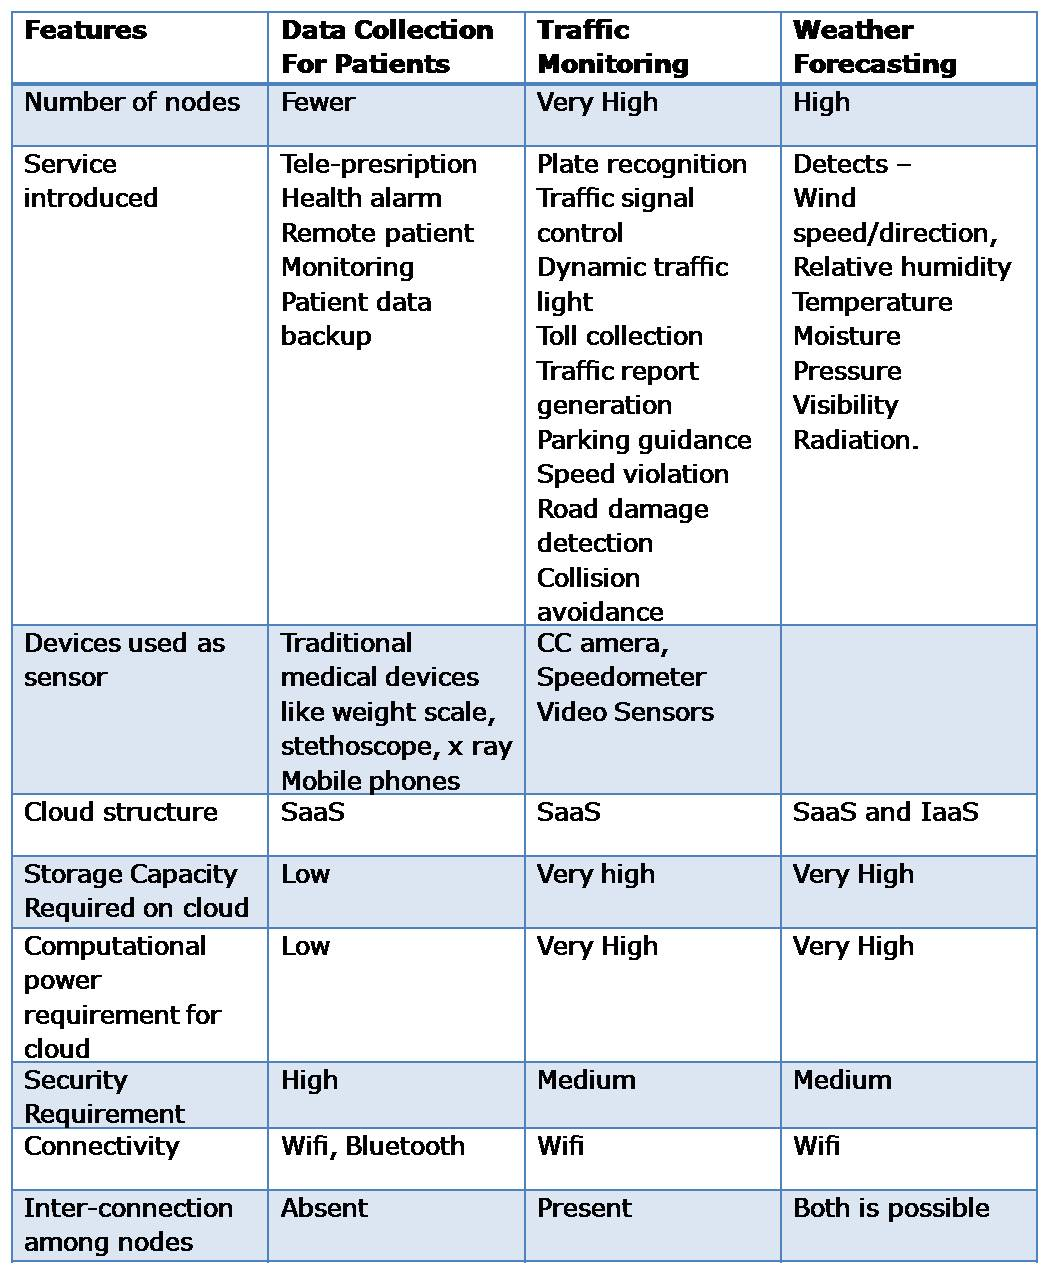
\includegraphics [scale=0.48]{table3}
\caption{Application of Cloud Computing For Sensor Network}
\end{center}
\end{figure}
%\newpage

\subsection{Traffic Monitoring}
Transport monitoring includes services like number plate recognition, traffic signal control, dynamic traffic light, toll collection, traffic report generation, parking guidance [12].
It can be used for legal and security purposes like speed violation, road damage detection, collision avoidance. Sensor devices with embedded network capability can be installed in roadside, speed breaker, on road and along with traffic light to detect and count vehicle.\\
\indent Traditional devices like cc amera, speedometer can be used for some sensing operations [12].The sensor will communicate with the neighboring nodes to develop a global picture.
Video Sensors can be made to detect potential crime scenes like burglary, street fight, suspicious dealings where otherwise large police deployment would be required.\\
\indent The above the applications require huge amount of storage capacity and computational ability.They also demand the need for extensive analysis of data for future prediction( for traffic monitoring [12]).
The application of cloud computing technology enables the system with very large storage and computational ability thus reducing the need for hardware establishment.The system is scalable and can offer complete analysis of data and is easy to access from any place.\\

\subsection{Weather Forecasting}
Weather forecasting is the application to anticipate the future atmosphere for a fixed location and time.Each weather station with sensors
 have the following detection ability - wind speed/direction, relative humidity, temperature, moisture, pressure, visibility and radiation.
The collected data is difficult to maintain using the traditional database approaches for it size.Assimilation is done after collecting the data.The complicated equations to predict future weather require super computer.\\


\subsection{Military surveillence}

	The integration can be used to collect wartime enviornmental information.sensor can be used to collect mine information.this can be used to detect and diffuse mine from remote place.


\chapter{Challenges}

{\bfseries \emph{Security:}\\}  One of the challenges of cloud computing lies in ensuring security and data integrity.Data integrity refers to maintaining and assuring the accuracy and consistency of data over its entire life-cycle. Data of cloud is at risk when at rest or during transition from sensor to cloud. As it is based completely on internet the risk of data exploitation is high. Data can be accessed and exploited by hack attack.Instead of attacking cloud hackers attack individual account.Though cloud is increasing its security, hackers are using more sophisticated method to attack [15].The scary thing is the vulnerability to Distributed Denial of Service (DDoS) attacks and the concentration of so much data,The single point of failure is the cloud. If something goes bad it impacts a very wide group of people. It's easier to steal and disrupt in bulk [15].



{\bfseries \emph{Privacy:}\\}
In cloud computing data is at the hand or cloud authority. The data can be stored on different geographical location. The client usually unaware of the data location. There is limited privacy of data since data is at the hand of third party, cloud authority.SLA (Service level Agreement) can be signed to ensure different level of security at different level.Senor collects the data,hands the data to cloud through data channel and cloud provide user with data in organized form and renders service.Through this process client is allowing cloud to access all sorts of data. So,data is not maintained as private to cloud owner.\\


{\bfseries \emph{Multipath fading:}\\} Multipath fading known as self interference when the two signals one is signal that is transmitted from a sensor and the other signal is the source signal bounced off from object interfere and two signals reach the destination at the same time. \\
Multipath fading occurs where multipath propagation in sensor network is. It can occur in wide range of signals including VHF and UHF. It is experienced in radio and cellular communication.

The possible scenario-\\

\begin{enumerate}
\item A sensor sends signal through a path.
\item Duplicate signal propagates though another path.
\item Second signal falls on an object.
\item Obstructed signal is reflected and sent to the sink
\item1st signal and second signal collide and one fades another. Sometimes signal completely fades away and falls below usable signal strength [14].Other times fading does not occur.
\end{enumerate}

\begin{figure}
%\centering
\begin{center}
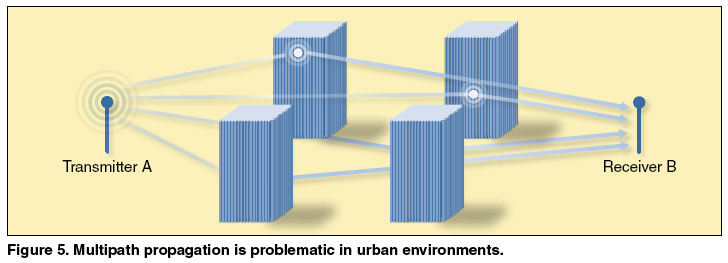
\includegraphics [scale=0.5]{multipath_fading}
\caption{Multipath Fading}
\end{center}
\end{figure}
%\newpage
\emph{Problems:} – Causes phase distortion and inter symbol interference [14] in radio signal\\
Below two types of fading-\\
{\bfseries Flat fading}-All signal of different frequency affected equally. Signal will change in amplitude [14].\\
{\bfseries Selective fading}-Signals of different frequency affected at a varying degree. Phase and amplitude [14] will vary.\\

{\bfseries \emph{Sensor Network expansion:}\\}Sensor network expansion is difficult to achive. If one need to deploy more sensors for the environment then it is costly and troublesome to extend the service of active sensors.If we want to enable sensor expansion or sensor shrinking ,then we have to keep  a large pool of sensors. Some of the sensors will be active while others will be inactive.



 When from cloud service a client demands for sensory data of locations of inactive sensors, then one have to request for sensor activation in those areas. Upon request from client through cloud sensors will be activated. Data of corresponding place will be available. But accessing sensor without virtualization will cause chaos and device dysfunction of sensors. 

\begin{figure}
%\centering
\begin{center}
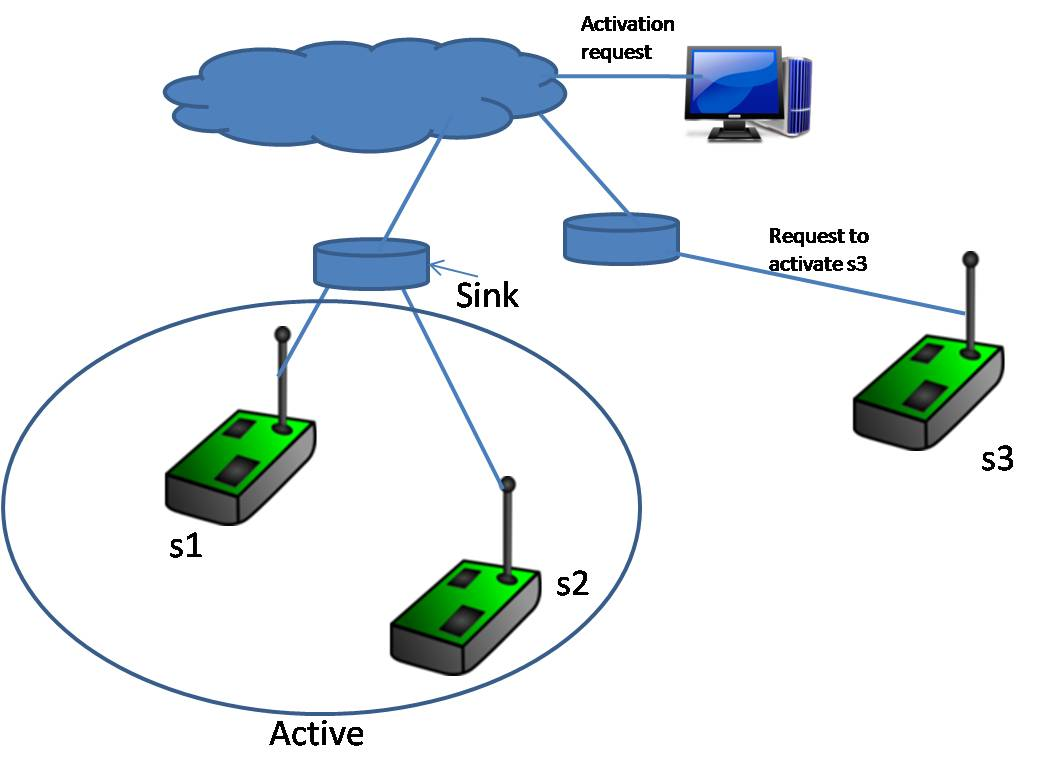
\includegraphics [scale=0.5]{expansion}
\caption{expansion}
\end{center}
\end{figure}
\newpage
So a level of virtualization is required for handling sensor and configuration. Achieving this is troublesome.\\


{\bfseries \emph{Interference:}\\}  Signal interference can occur if two sensors send signal at the same time and through same

\begin{figure}
%\centering
\begin{center}
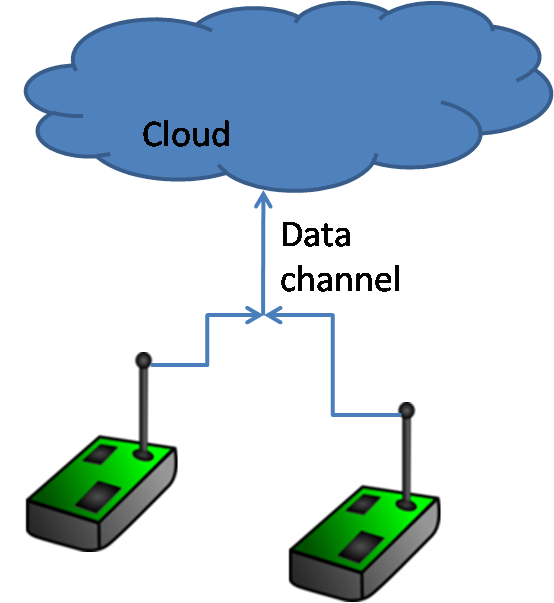
\includegraphics [scale=0.5]{interference}
\caption{Interference}
\end{center}
\end{figure}
\newpage

 channel. The two sensor node can be from same network or from different WSNs.Interference is a phenomenon in which two signals superimpose to form a resultant wave of greater or lower amplitude. \\




{\bfseries \emph{Data Fusion:}\\} Sensor collects heterogenous data.To optimize the data,data fusion can be addressed as solution.Data fusion is the process of integration of multiple data and knowledge representing the same real-world object into a consistent, accurate, and useful representation [13].Chosing the right data fusion technique for sensor network is a challange.

{\bfseries \emph{Service Downtime and Hardware Maintenance :}\\} Exact location of data is unknown so; data recovery after disaster is difficult. Outage is another problem. Most reliable cloud can have downtime when they are unable to provide services. The cloud service is dependent on health of cloud system and underlying hardware health. If for any reason the hardware fail to stay in good state the system will fall down.\\

{\bfseries \emph{Device Configuration:}\\}\indent If cloud software is updated than installed application in client device has to be updated too. Any incompatibility may result in service failure.\\

\chapter{Challenges of sensor virtualization}

Embedding of virtual sensor networks, with constraints on nodes and links, can be reduced to the NP-hard problem even when all virtual network requests are known in advance.\\

{\bfseries \emph{Heterogenous sensor device:}\\}Sensor network nodes can be of varying types and data found from sensor can be heterogeneous. Interface of virtual sensor should be implemented considering this feature.More over resource topology and device status has to be understood. 

{\bfseries \emph{QoS:}\\}In virtualization, quality of service and quality of experience is important but hard to manage. Quality of service depends on health of the network and devices. Quality of experience depends on user level experience.

{\bfseries \emph{Resource Constraint:}\\}Sensor nodes are resource constraint. Virtual sensor should be developed keeping this in mind. 

\begin{figure}
%\centering
\begin{center}
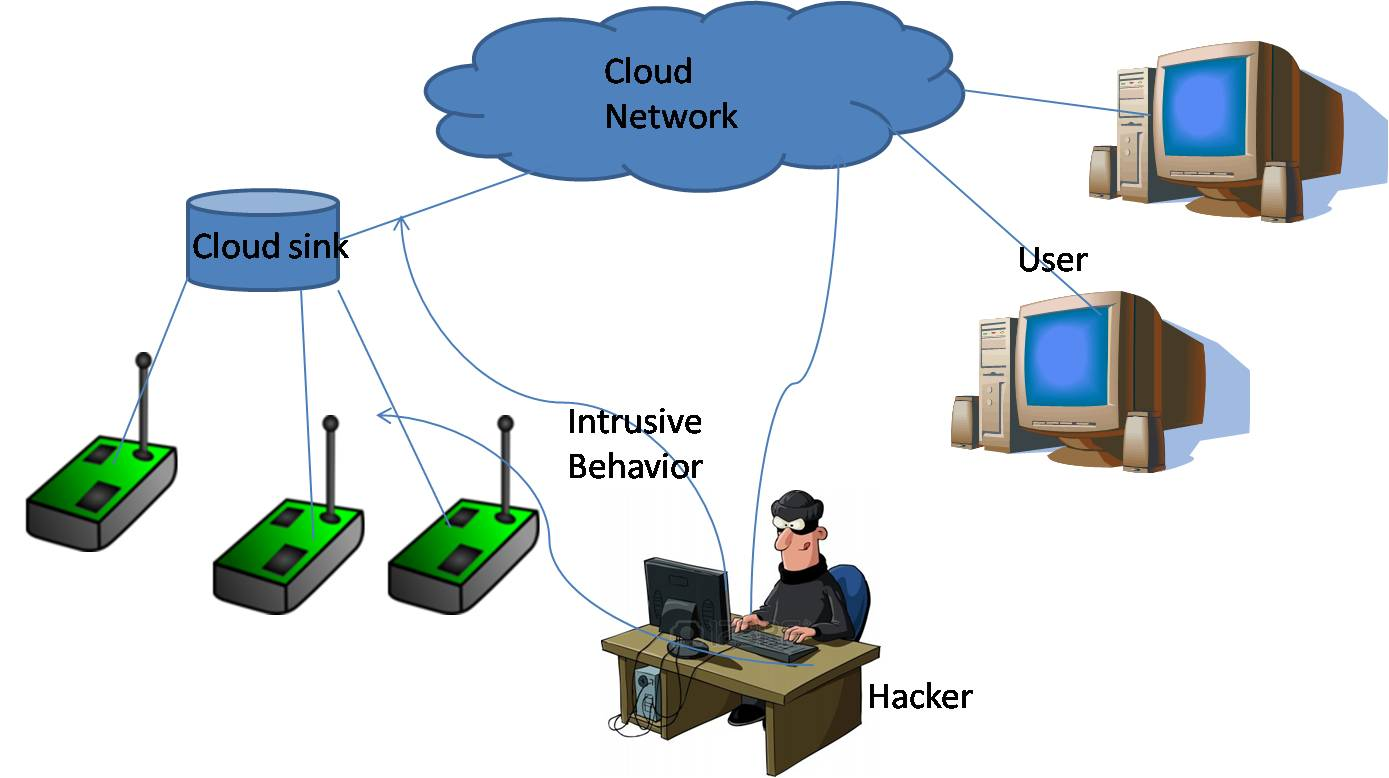
\includegraphics [scale=0.5]{hack2}
\caption{Hack Attack}
\end{center}
\end{figure}
\newpage

{\bfseries \emph{Secuirity:}\\}Assuring high level security is essential. Security failure may result in system exploitation as data from sensor is requires guarantee of confidentiality. Misuse of accessed data and ill-handling will cause major privacy and security issue.A Hacker can leak data while transmisson going on between sensor and sink node,during sink to cloud transmission and at the time of cloud user exchange.During this 3 types of tranmission process data is at risk of exploitation.This way Data can be altered ,sensors can be damaged and user will experience service disruption.\\


{\bfseries \emph{Infrastructure problem:}\\}There are two types of infrastructure. Physical sensor infrastructure and virtual sensor infrastructure.Owner of the two infrastructure may be different and have buyer seller relationship.Aplication level user is also a buyer of the provided service. Two types of market place -centralized and decentralized. Centralized market place is not scalable, prone to attack but efficient. Decentralized one is fault tolerant but prone to abnormal behavior.

{\bfseries \emph{Redundant provision:}\\}
User provision must not exceed the capacity of network.

\begin{figure}
%\centering
\begin{center}
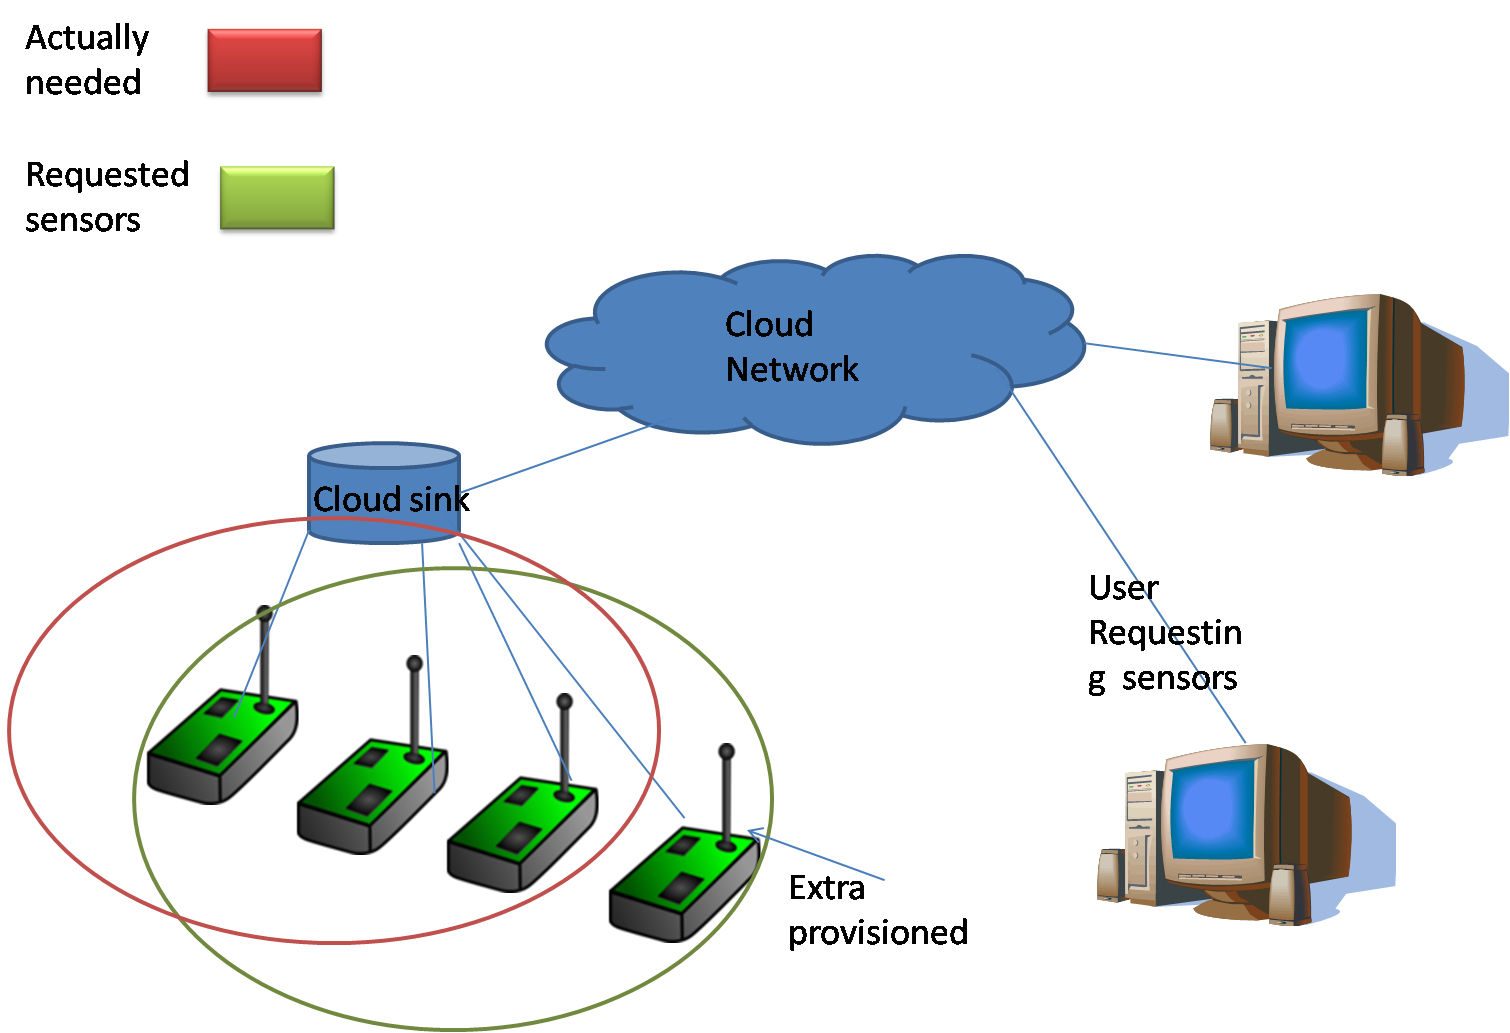
\includegraphics [scale=0.5]{prov}
\caption{Hack Attack}
\end{center}
\end{figure}
\newpage

 It has to be made sure that the user don’t occupy more than resource allocation. Exploiting virtual sensor by user has to be prevented. \\

{\bfseries \emph{Sensor Exploitation:}\\}
Failure in physical link will cause failure in virtual links. Failure in physical sensor may result in failure in multiple virtual sensors.\\

{\bfseries \emph{Energy Constraint:}\\}
 Sensors have energy constraint .While allocating sensors for service system have to be able to handle when sensors reach power constraint. Based on energy level sensors have to be put on rest.Taking proper step during outage is challanenging.\\



\chapter{Conclusion}
In this paper,we defined the terminologies and classifications of Cloud and Sensor Network.The article intends to shift towards making sensor more service oriented towards the application of sensing in real life.
The idea is to make sensor data widely accessible  and comprehensible to the user.The proposed technology can enhance user experience on corporate and personal level.
Application of cloud technology will make sensor data widely accessible and open to complex data analysis and provide sensor data as service.






\begin{thebibliography}{samplelabel}

\bibitem[1]{ Jayashree } Jayashree, J.; Vijayashree J.; Ubiquitous Life Care Integrates Wireless Sensor Network And Cloud Computing With Security ;Global Journal of  Computer Science and Technology, 2011.
\bibitem[2]{ Rolim} Rolim, C .O; Koch, F.L; Westphall, C.B; A Cloud Computing Solution for Patient's Data Collection in Health Care Institutions.
\bibitem[3]{Sheng} Sheng, X.; Xiao, X.; Tang,J.;Xue, G.; Sensing as a Service: A Cloud Computing System for Mobile Phone Sensing.
\bibitem[4]{Sun} Sun H. ;Zhang.P.;Yan Z.; A Novel Architecture Based on Cloud Computing for Wireless Sensor Network  (ICCSEE 2013).
\bibitem[5]{Duan} L. Duan; et al.; Incentive mechanisms for smart phone collaboration in data acquisition and distributed computing, IEEE Infocom’2012.
\bibitem[6]{Mitton} Mitton, N.; Papavassiliou, S.; Puliafito, A.;Trived, K.; Combining Cloud and sensors in a smart city Environment (2012).
\bibitem[7]{Wang} Wang, W.; Lee, K., Murray, D.; Integrating Sensors with the Cloud Using Dynamic Proxies.
\bibitem[8]{Lounis} Lounis, A.;  Hadjidj, A.;Bouabdallah, A.; Challal, Y.; Secure and Scalable Cloud-based Architecture for e-Health Wireless sensor networks.
\bibitem[9]{Goyal}Goyal, A.;  Dadizadeh, S. ; A Survey on Cloud Computing.
\bibitem[10]{Lee} Lee,K.;Murray,D.;Hughes,D.;Joosen,W;Extending Sensor Networks into the Cloud using Amazon Web Services.pp.6-7
\bibitem[11]{Cloud_computing}\url{http://en.wikipedia.org/wiki/Cloud_computing}
\bibitem[12]{Sanjit}Dash,S.K.; Mohapatra,S.;  Pattnaik,P.K.; A Survey on Applications of Wireless Sensor Network Using Cloud Computing ,December 2010, pp.1-2
\bibitem[13]{Data fusion} \url{http://en.wikipedia.org/wiki/Data_fusion}
\bibitem[14]{Multipath-fading}\url{ http://www.radio-electronics.com/info/propagation/multipath/multipath-fading.php}
\bibitem[15]{Dangers of cloud}\url{http://www.businessnewsdaily.com/5215-dangers-cloud-computing.html}
\bibitem[16]{Islam}  Islam,M.,M.;  Hassan,M.,M.; Lee,G.; Huh,E.;A Survey on Virtualization of Wireless Sensor Networks,Feb 15, 2012.


\end{thebibliography}

\end{document}



